\documentclass{beamer}
\usepackage[utf8]{inputenc}
\usepackage[english, russian]{babel}
\usepackage{amsmath,mathrsfs,mathtext}
\usepackage{graphicx, epsfig}
\usepackage{caption}
\usepackage{subfig}
\usepackage{amsmath, bm}

\usepackage{tikz}

\DeclareMathOperator*{\argmin}{arg\,min}
\DeclareMathOperator*{\argmax}{arg\,max}

\makeatletter
\let\@@magyar@captionfix\relax
\makeatother

\usetheme{Warsaw}
\usecolortheme{sidebartab}
\definecolor{beamer@blendedblue}{RGB}{31,96,49}

%----------------------------------------------------------------------------------------------------------
\title[\hbox to 56mm{Локальная кластеризация временных рядов \hfill\insertframenumber\,/\,\inserttotalframenumber}]
{Локальная кластеризация временных рядов}
\author[Грабовой А. В.]{\large Грабовой Андрей}
\institute{\large Московский физико-технический институт\\
Факультет управления и прикладной математики\\
Кафедра интеллектуальных систем\\
~\\
Научный руководитель д.ф.-м.н. В. В. Стрижов
}

\date{\footnotesize{\emph{Москва,}\\
 2019г}}
%----------------------------------------------------------------------------------------------------------
\begin{document}
%----------------------------------------------------------------------------------------------------------
\begin{frame}
\titlepage
\end{frame}
%----------------------------------------------------------------------------------------------------------
\begin{frame}{Цель работы}
	\begin{block}{Исследуется}
		Исследуется задача распознавания характерных периодических сигналов внутри временного ряда. 
	\end{block}
	
	\begin{block}{Требуется}
		Требуется предложить признаковое описание моментов времени ряда, для дальнейшей кластеризации точек данного ряда.
	\end{block}
	
	\begin{block}{Проблемы}
		Построение адекватного локального признакового описания временного ряда.
	\end{block}
\end{frame}
%----------------------------------------------------------------------------------------------------------
\begin{frame}{Список литературы}
	\begin{itemize}
		\item \textit{И. П. Ивкин,  М. П. Кузнецов} Алгоритм классификации временных рядов акселерометра по комбинированному признаковому описанию.~// Машинное обучение и анализ данных, 2015.
		\item \textit{V. V. Strijov, A. M. Katrutsa} Stresstes procedures for features selection algorithms.~// Schemometrics and Intelligent Laboratory System, 2015.
		\item \textit{T. Kanungo, D. M. Mount et al} An Efficient k-Means Clustering Algorithm: Analysis and Implementation. 2000.
		\item \textit{I. Borg, P. J. F. Groenen} Modern Multidimensional Scaling. --- New York: Springer, 2005. 540 p.
		\item \textit{Д. Л. Данилова, А. А. Жигловский} Главные компоненты временных рядов: метод "Гусеница". --- СПбУ, 1997.
	\end{itemize}
\end{frame}
%----------------------------------------------------------------------------------------------------------
\begin{frame}{Постановка задачи}
Задан временной ряд:
$$\textbf{X} \in \mathbb{R}^{\text{N}\times 1}, \quad \textbf{X} = [\textbf{v}_1, \textbf{v}_2, \cdots, \textbf{v}_M], \quad \textbf{v}_i \in \mathcal{V},$$
где $\mathcal{V}$ некоторое множество возможных сигналов.

~\\
Предположения:
\begin{itemize}
	\item $\left|\mathcal{V}\right| = K$,
	\item $\forall \textbf{v} \in \mathcal{V}~\left|\textbf{v}\right| \leq T$,
	\item $\forall i$ выполняется $\textbf{v}_i = \textbf{v}_{i-1}$ или   $\textbf{v}_i = \textbf{v}_{i+1}$,
\end{itemize}
где $\left|\mathcal{V}\right|$ мощность множества сигналов, а $\left|\textbf{v}\right|$ длина сигнала.

\end{frame}
%----------------------------------------------------------------------------------------------------------
\begin{frame}{Постановка задачи}
Рассмотрим отображение:
$$a : x \to \{1,\cdots, K\}$$
где $x \in \textbf{X}$ некоторая точка временного ряда.

~\\
Потребуем следующие свойства:
$$
\begin{cases}
    a\left(x_1\right) = a\left(x_2\right), & \text{если}~\exists \textbf{v} \in \mathcal{V}: x_1,x_2 \in v\\
    a\left(x_1\right) \not= a\left(x_2\right), & \text{если}~\not\exists \textbf{v} \in \mathcal{V}: x_1,x_2 \in v
\end{cases}
$$

\end{frame}
%----------------------------------------------------------------------------------------------------------
\begin{frame}{Кластеризация точек}
Фазовая траектория ряда $\textbf{X}$:
$\mathcal{H} = \{\textbf{h}_t| \textbf{h}_t = [x_{t-T}, x_{t-T+1}, \cdots, x_{t}],~\text{T}\leq t\leq \text{N}\}.$

~\\
Фазовые подпространства:
$\mathcal{S} = \{\textbf{s}_t| \textbf{s}_t = [h_{t-2T}, h_{t-2T+1}, \cdots, h_{t}],~\text{2T}\leq t\leq \text{N}\}.$

~\\
Пространство базисов:
$$\mathcal{W} = \{\textbf{W}_{t}| \textbf{W}_t = [\textbf{w}^1_t, \textbf{w}^2_t]\}, \quad \mathcal{L} = \{\bm{\lambda}_t| \bm{\lambda}_t=[\lambda^1_t, \lambda^2_t]\}, $$
где $[\textbf{w}^1_t, \textbf{w}^2_t]$ и $[\lambda^1_t, \lambda^2_t]$ это базисные векторы и сингулярные числа метода главных компонент для подпространства $s_t$.
\end{frame}
%----------------------------------------------------------------------------------------------------------
\begin{frame}{Кластеризация точек}
Расстояние между элементами $\mathcal{W}$:\\
$\rho\left(\textbf{W}_1, \textbf{W}_2\right) = \max_{\{\textbf{a},\textbf{b},\textbf{c}\} \subset \textbf{W}_1\cup \textbf{W}_2 } V\left(\textbf{a},\textbf{b},\textbf{c}\right),$
где $V\left(\textbf{a},\textbf{b},\textbf{c}\right)$ --- объем паралелепипеда на $\textbf{a}, \textbf{b}, \textbf{c}$.

~\\
Расстояние между элементами $\mathcal{L}$:\\
$\rho\left(\bm{\lambda}_1, \bm{\lambda}_2\right) = \sqrt[]{\left(\bm{\lambda}_1 - \bm{\lambda}_2\right)^{\mathsf{T}}\left(\bm{\lambda}_1 - \bm{\lambda}_2\right)}.$

~\\
Расстояние между точками временного ряда:\\
$\rho\left(t_1, t_2\right) = \rho\left(\textbf{W}_1, \textbf{W}_2\right) + \rho\left(\bm{\lambda}_1, \bm{\lambda}_2\right).$

~\\
Матрица попарных растояний:\\
$\textbf{M} = [0, 1]^{N\times N}.$

\end{frame}
%----------------------------------------------------------------------------------------------------------
\begin{frame}{Эксперимент}
\begin{table}[h]
	\begin{center}
	\caption{Описание выборок}
		\begin{tabular}{|c|c|c|c|}
		\hline
			Выборка &N& K& T\\
			\hline
			\multicolumn{1}{|l|}{Real}
			& & & \\
			\hline
			\multicolumn{1}{|l|}{Synthetic 1}
			& 2000& 2& 20\\
			\hline
			\multicolumn{1}{|l|}{Synthetic 2}
			& 2000& 3& 20\\
		\hline
		\end{tabular}
	\end{center}
\end{table}
\end{frame}
%----------------------------------------------------------------------------------------------------------
\begin{frame}{Синтетические данные}
	\begin{figure}[h!t]\center
		\subfloat[Synthetic 1]{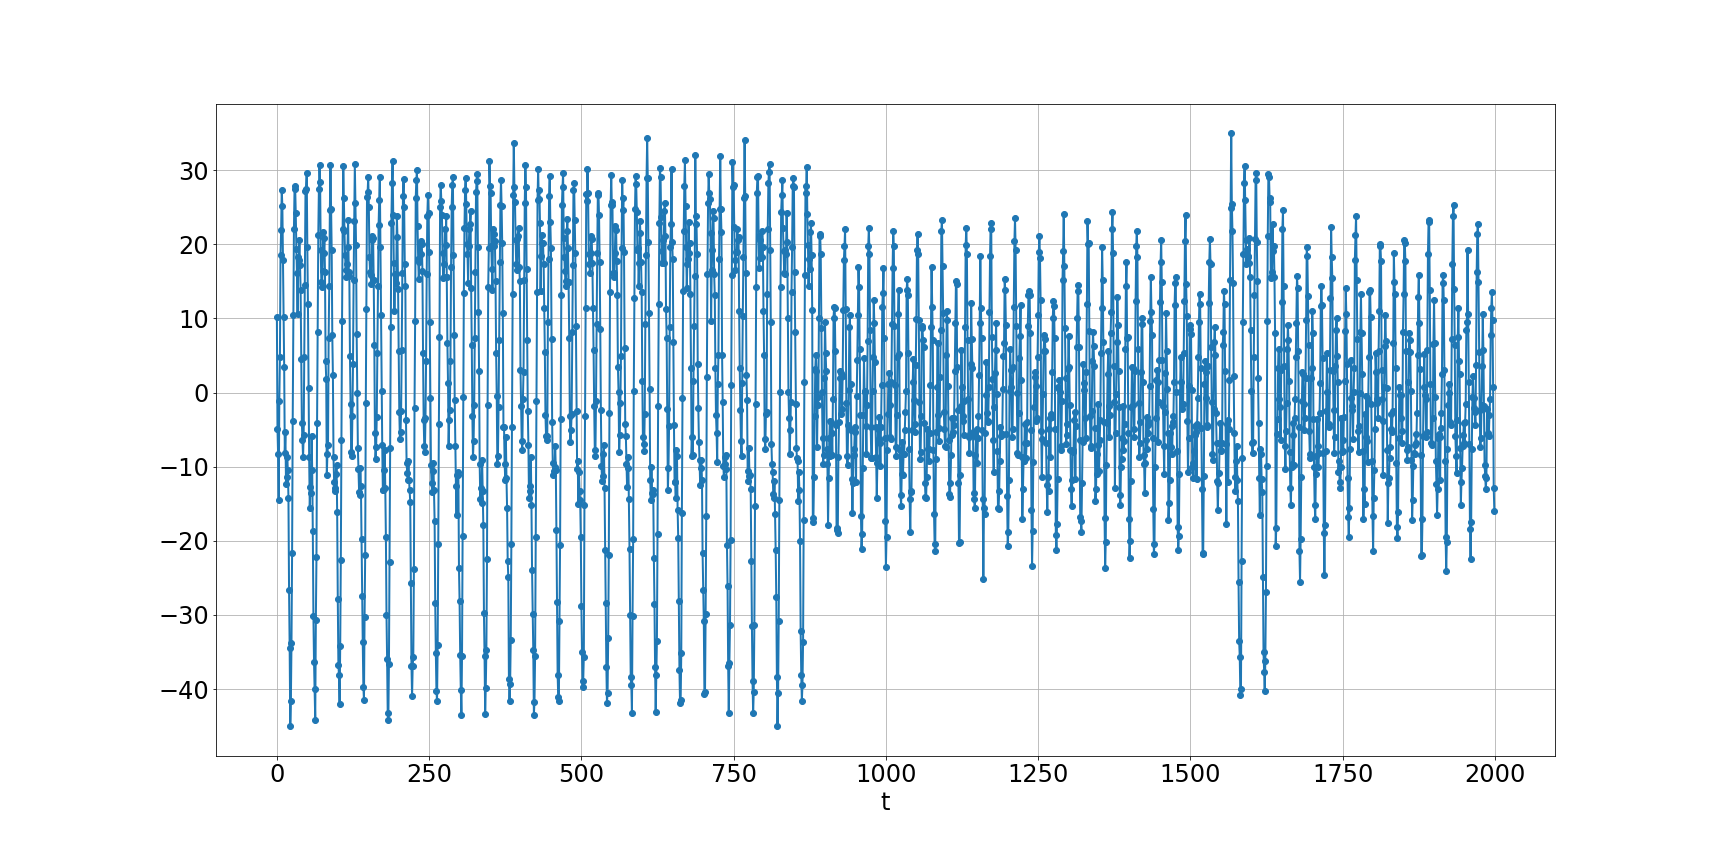
\includegraphics[width=0.5\textwidth]{results/2_patern_series}}
		\subfloat[Synthetic 2]{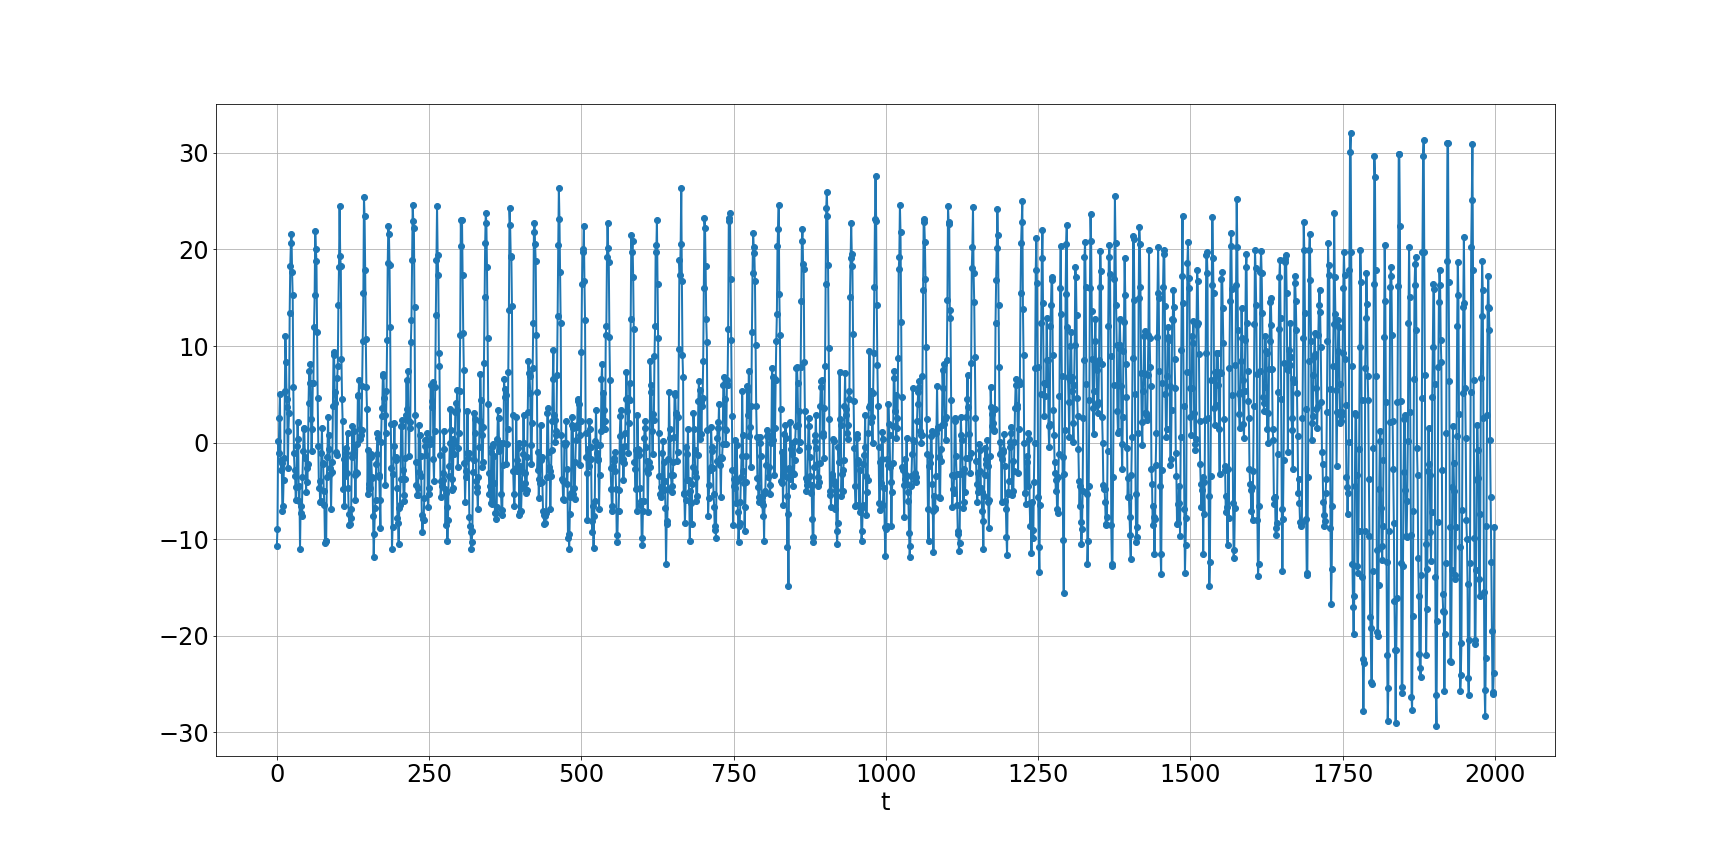
\includegraphics[width=0.5\textwidth]{results/3_patern_series}}\\
		\caption{Пример синтетически построенных временных рядов}
	\end{figure}
\end{frame}
%----------------------------------------------------------------------------------------------------------
\begin{frame}{Синтетические данные}
	\begin{figure}[h!t]\center
		\subfloat[Synthetic 1]{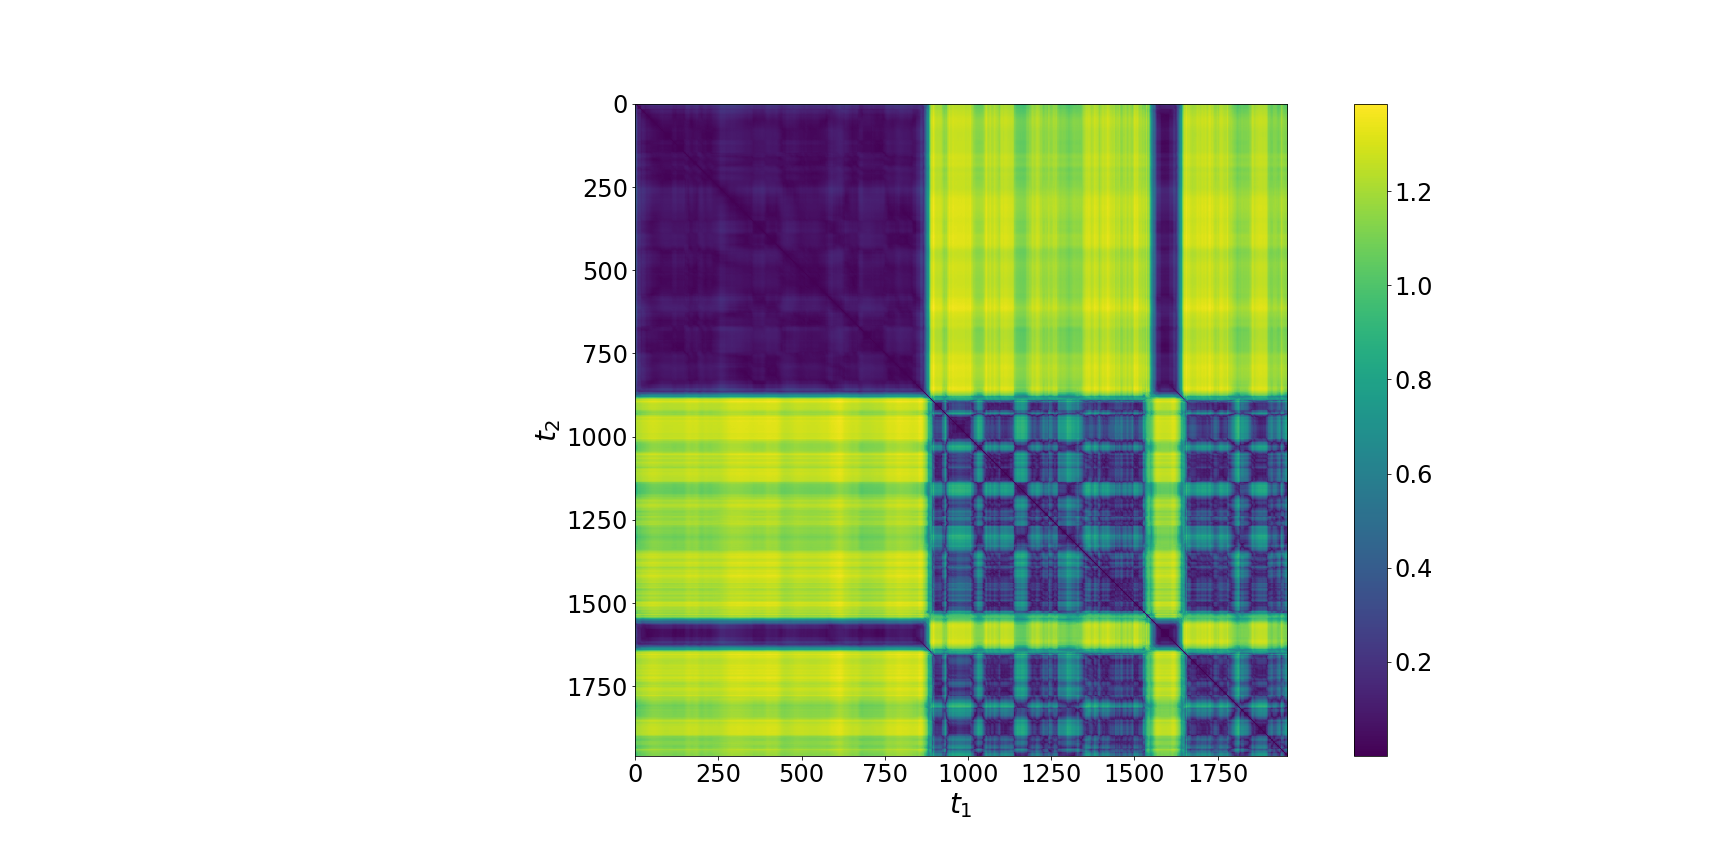
\includegraphics[width=0.5\textwidth]{results/2_patern_full}}
		\subfloat[Synthetic 2]{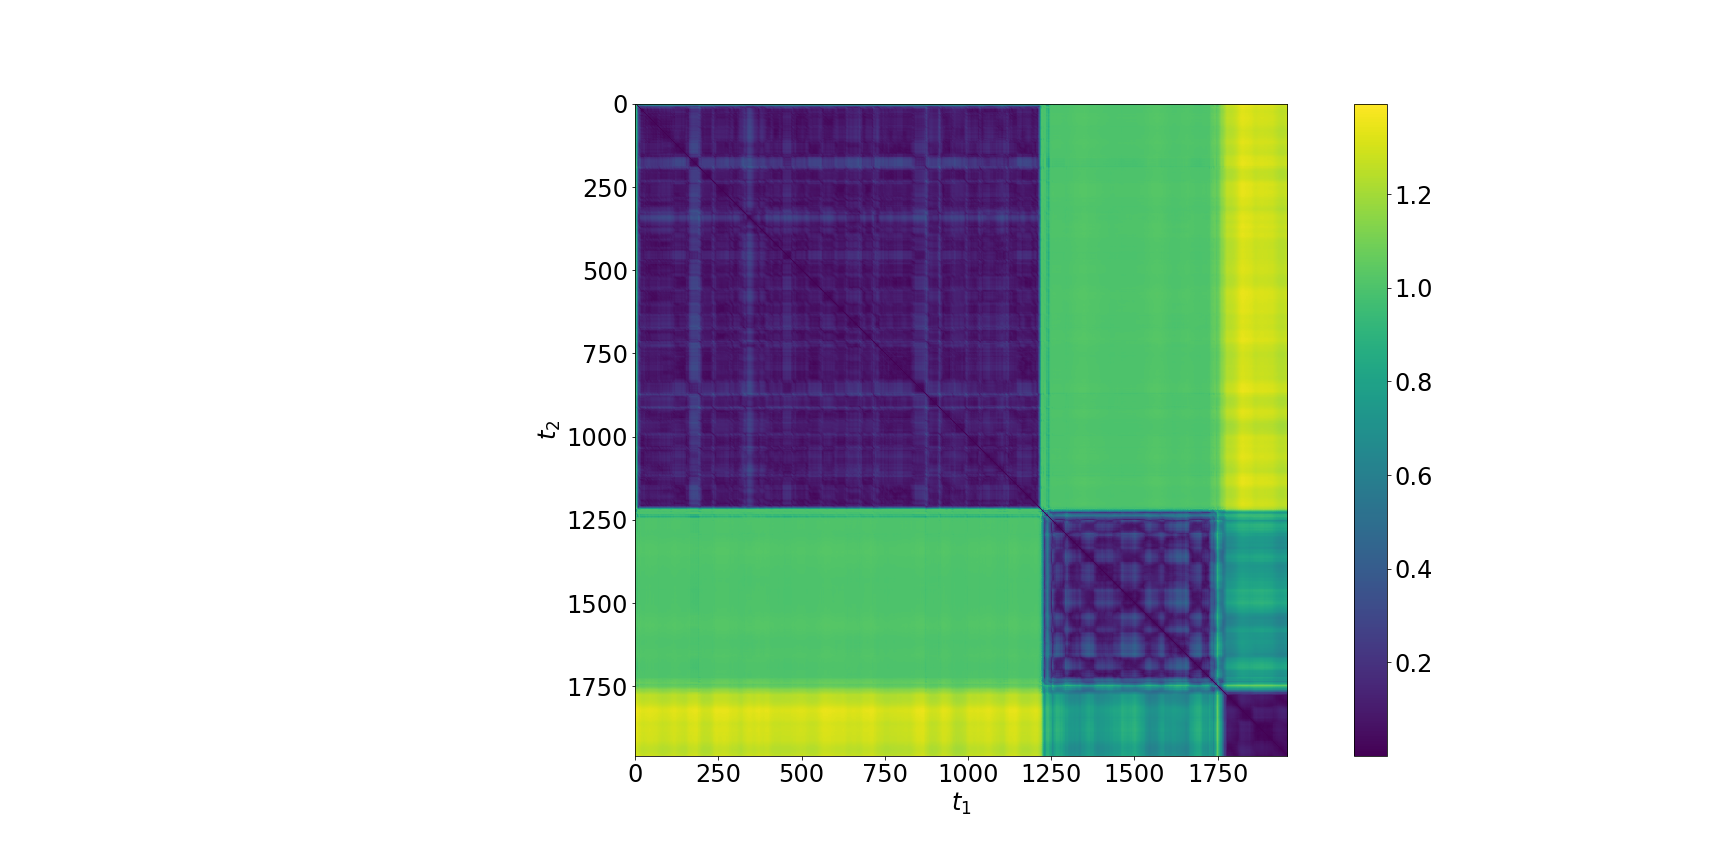
\includegraphics[width=0.5\textwidth]{results/3_patern_full}}\\
		\caption{Матрица попарных расстояний $\textbf{M}$ между точками временного ряда}
	\end{figure}
\end{frame}
%----------------------------------------------------------------------------------------------------------
\begin{frame}{Синтетические данные}
	\begin{figure}[h!t]\center
		\subfloat[Synthetic 1]{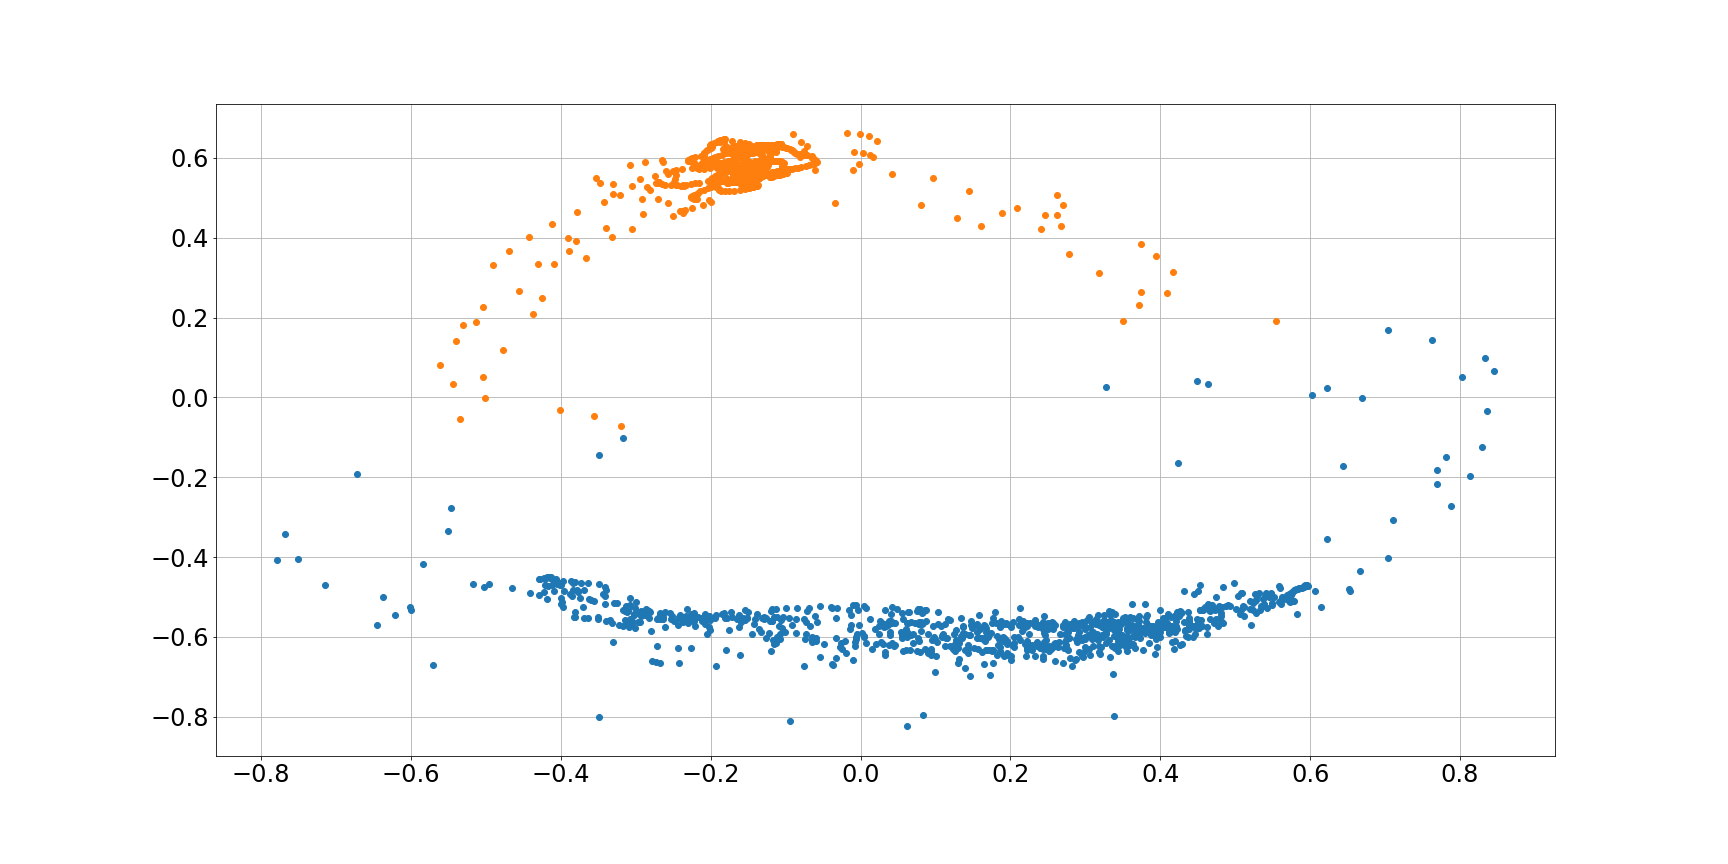
\includegraphics[width=0.5\textwidth]{results/2_patern_2D_vector}}
		\subfloat[Synthetic 2]{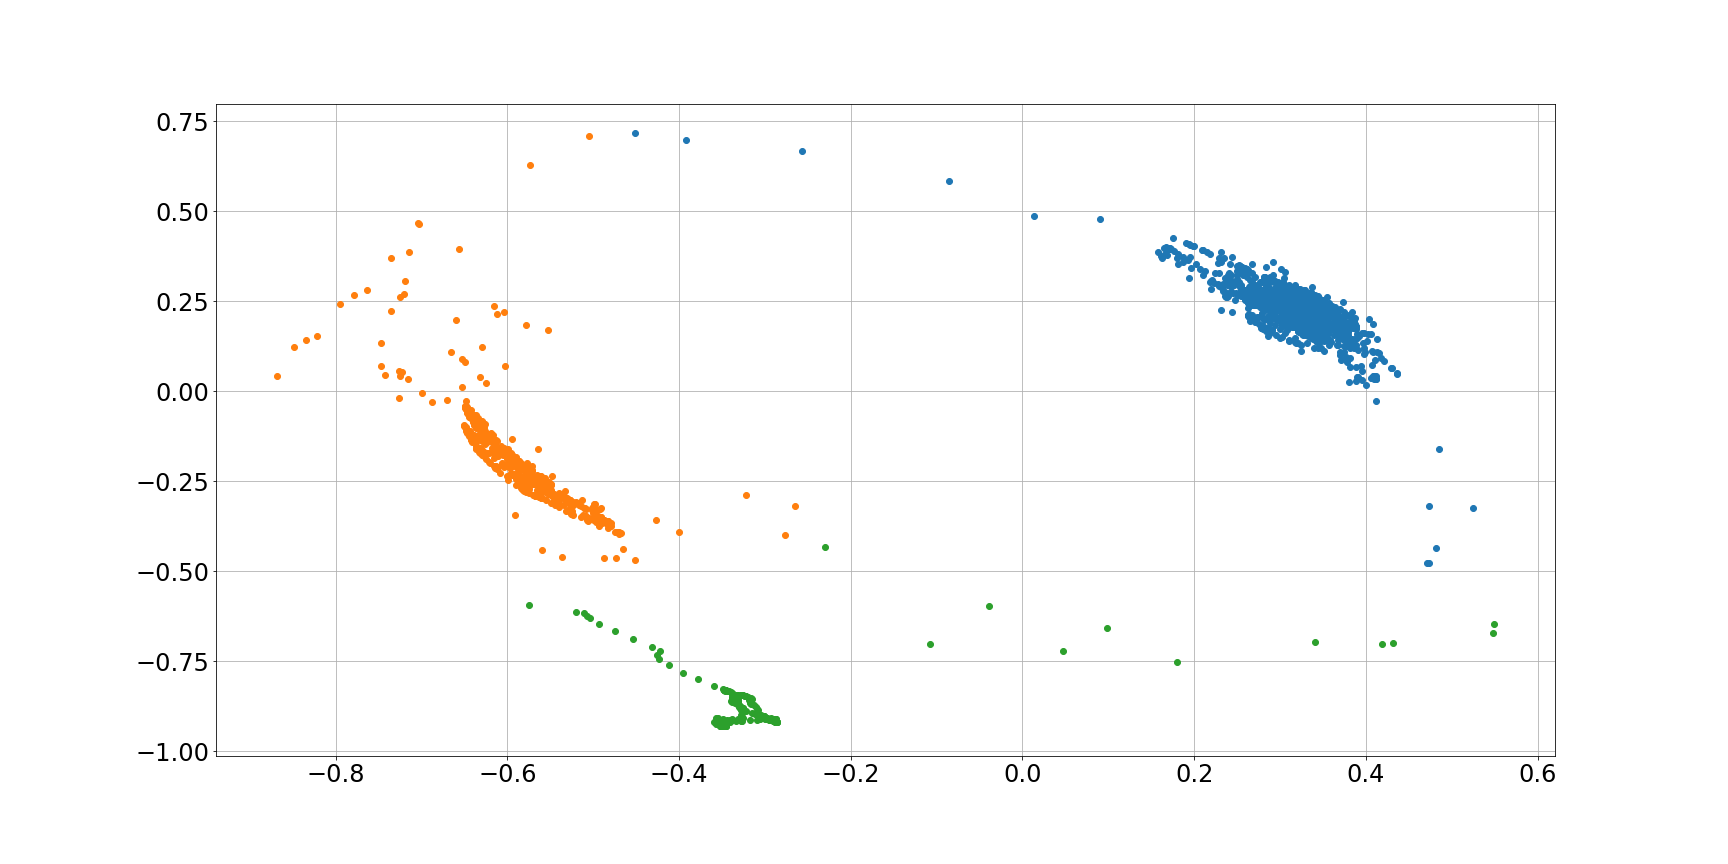
\includegraphics[width=0.5\textwidth]{results/3_patern_2D_vector}}\\
		\caption{Проекция точек временного на плоскость при помощи матрицы попарных расстояний $\textbf{M}$}
	\end{figure}
\end{frame}
%----------------------------------------------------------------------------------------------------------
\begin{frame}{Синтетические данные}
	\begin{figure}[h!t]\center
		\subfloat[Synthetic 1]{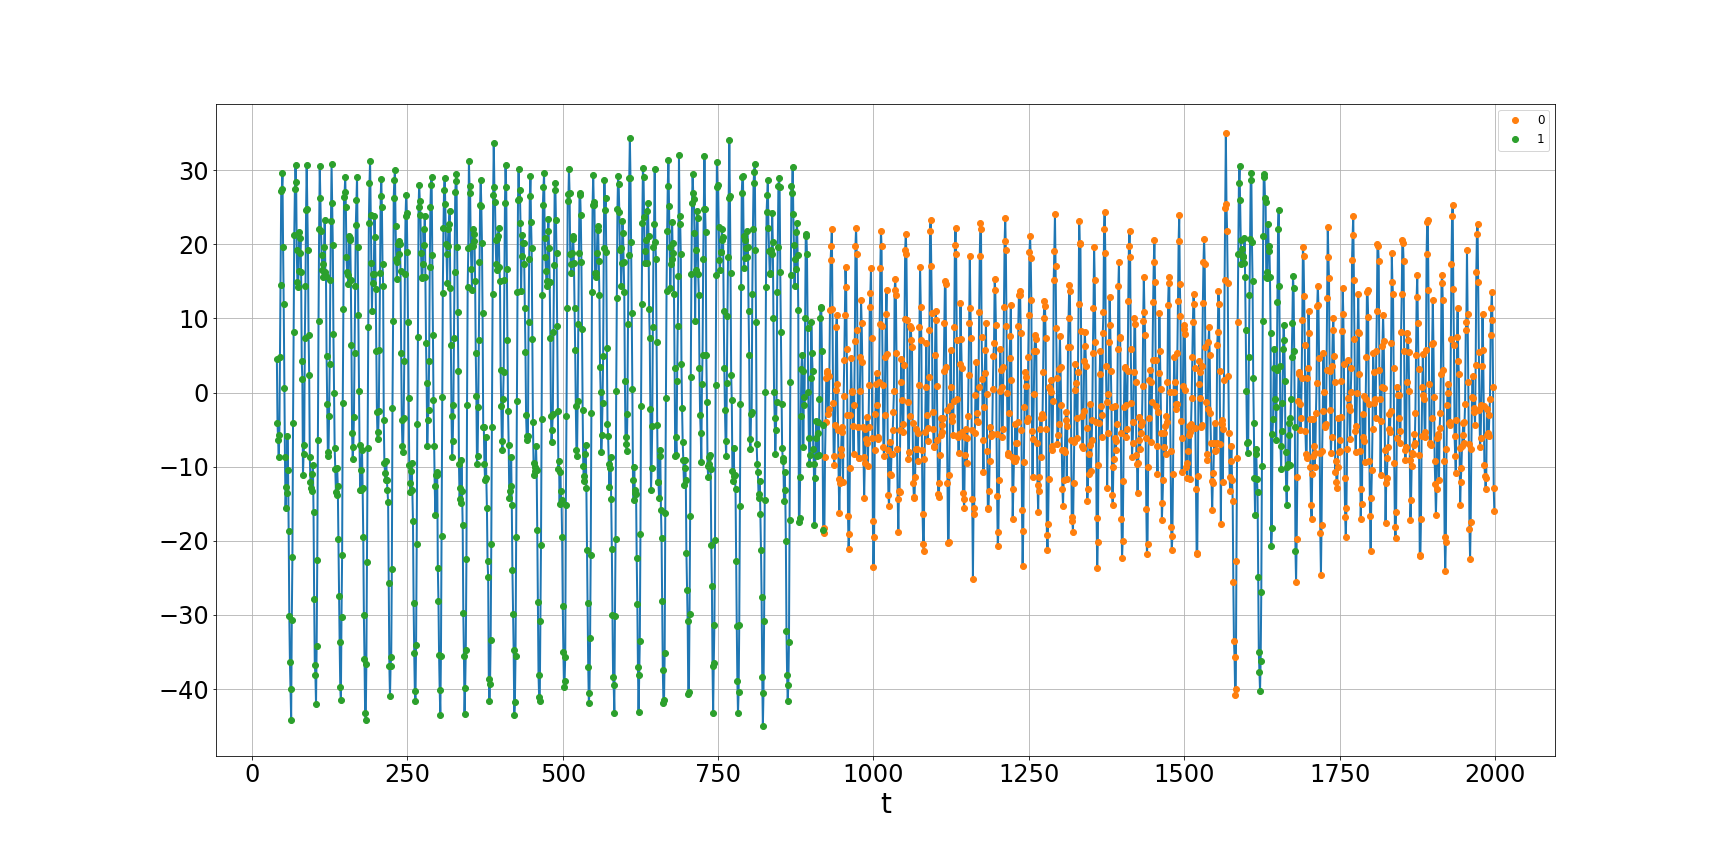
\includegraphics[width=0.5\textwidth]{results/2_patern_claster_vector}}
		\subfloat[Synthetic 2]{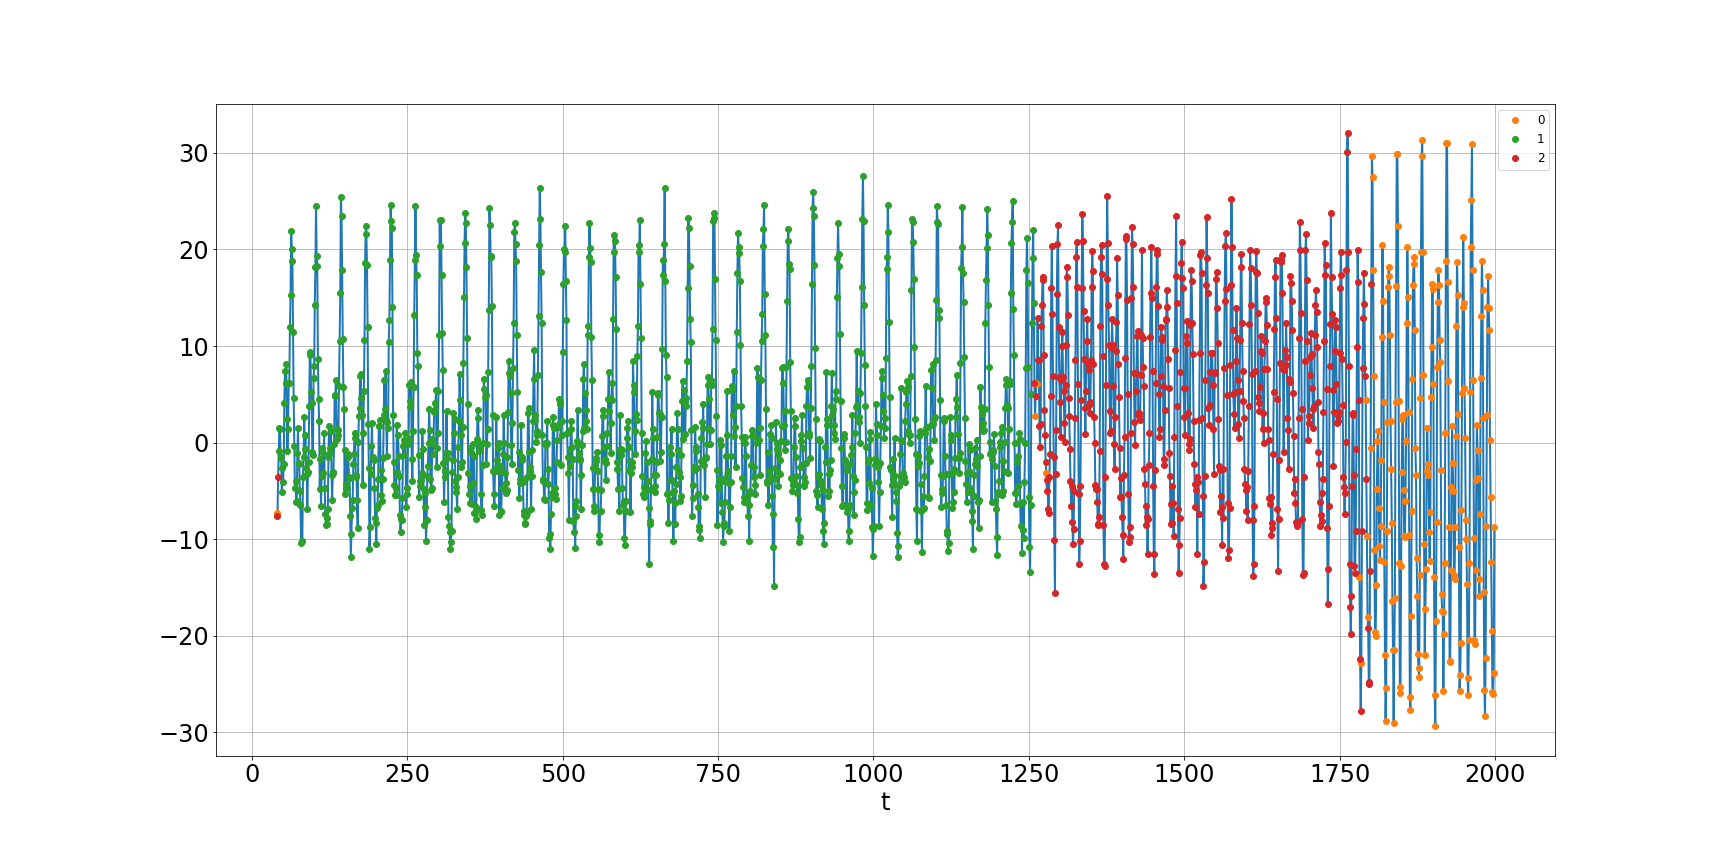
\includegraphics[width=0.5\textwidth]{results/3_patern_claster_vector}}\\
		\caption{Кластеризация точек временного ряда}
	\end{figure}
\end{frame}
%----------------------------------------------------------------------------------------------------------
\begin{frame}{Публикации по теме}
	
\end{frame}
%----------------------------------------------------------------------------------------------------------
\begin{frame}{Заключение}
	\begin{itemize}
		\item Был предложен алгоритм поиска характерных сигналов, который основывается на методе главных компонент для локального снижения размерности.
		\item Была предложена функция расстояния между локальными базисами в каждый момент времени, которые интерпретировались как признакового описание точки временного ряда.
		\item Предложенный алгоритм хорошо разделяет точки которые принадлежат разным классам сигналов, что хорошо для кластеризации точек временного ряда.
	\end{itemize}
\end{frame}
%----------------------------------------------------------------------------------------------------------

\end{document} 